\section{Resultados e discussões}

\subsection{Anel de Gravesande}
Ao realizar o experimento do Anel de Gravesande, observou-se que, à temperatura ambiente, a esfera metálica passava justamente através do anel. Após o aquecimento da esfera utilizando um pequeno balão cheio de álcool e com um pavio, notou-se que a esfera não conseguia mais atravessar o anel. Ao deixar a esfera esfriar por alguns instantes, ela voltava a passar pelo anel.

O funcionamento do Anel de Gravesande é uma demonstração clássica do fenômeno da dilatação térmica volumétrica dos sólidos. Em que quando um material é aquecido, a energia térmica fornecida aumenta a energia inética média de seus átomos e moléculas. Isso faz com que eles vibrem com maior amplitude, resultado em um aumento médio nas distancias interatômicas e, consequentemente, na expansão do volume do material.

Tal dilatação volumétrica (\(\Delta V\)) pode ser aproximada pela seguinte relação:
\begin{align*}
	\Delta V = V_0 * \gamma * \Delta T
\end{align*}
sendo, \(V_0\) o volume inicial do objeto, \(\gamma\) é o coeficiente de dilatação volumétrica do material e \(\Delta T\) é a variação de temperatura.

No caso do experimento realizado, a esfera era pequena, em uma ordem de, no máximo, uma dezena de centímetros, e o aquecimento da esfera, por ter sido realizado por pouco tempo e com uma pequena fonte de calor, a alteração de volume na esfera, foi de menos que um centímetro ao quadrado o que já foi o suficiente para impedir a passagem da esfera pelo anel.

Por fim, essa dinâmica física da dilatação térmica  volumétrica, é vastamente utilizada em diversas áreas da sociedade atual. Alguns exemplos mais práticos, é a utilização dessa dinâmica para a área industrial, para melhor encaixe de peças, e para a de resistência de alguns materiais, outro exemplo bem palpável é a utilização de termômetros de mercúrio, em que seu funcionamento se baseia na dilatação térmica do mercúrio em uma ampola graduada.  

\subsection{Par Bimetálico}
No experimento do par bimetálico, foi observado que, ao aquecer a lâmina bimetálica torcida, observou-se que a lâmina se esticava rapidamente, fazendo com que fosse puxado o ponteiro que estava na extremidade livre, assim fazendo-o movimentar e encostar na outra fase. Ao deixar a lâmina bimetálica esfriar por alguns instantes, observou-se que ela voltou à torção original, com o ponteiro para baixo, na fase inicial.

O funcionamento físico desse experimento do par bimetálico baseia-se na diferença do coeficiente de dilatação linear de dois metais distintos, que compõem a lâmina. Dessa forma, quando a lâmina é aquecida, ambos os metais tentam se expandir. No entanto, o metal com maior coeficiente de dilatação (\(\alpha_1\)) tenderá  a se expandir mais do que o metal com menor coeficiente de dilatação(\(\alpha_2\)) para a mesma variação de temperatura(\(\Delta T\)).

Como os dois metais estão unidos, eles não podem se expandir livremente de forma independente. Para acomodar essa diferença de expansão, a lâmina se curva para o lado que compõe o metal que possui o menor coeficiente de dilatação linear. Dessa forma, como a lamina estava enrolada, e ao aquecê-la, observou-se uma diminuição na torção, é possível dizer que a composição da lamina bimetálica tinha o metal com maior coeficiente de dilatação para fora, mostrado com a cor azul na Figura \cref{ParBimetalico}

\begin{figure}[H]
	\centering
	\includegraphics[width=0.25\linewidth]{fig/ParBimetálico.png}
	\caption{Lâmina bimetálica fixa composta por dois metais, representados pelas cores azul e vermelho, e ponteiro representado com verde. Fonte: Autoria própria.}
	\label{ParBimetalico}
\end{figure}

A capacidade do par bimetálico de se curvar de forma previsível com as mudanças de temperatura o torna muito útil em diversas aplicações práticas. Seu uso mais conhecido é em termostatos, onde funciona para controlar a temperatura em sistemas de ar condicionado, aquecedores e refrigeradores. Além disso, essa deformação causada pelo calor é o princípio de funcionamento de termômetros analógicos e de disjuntores térmicos, que são essenciais para proteger circuitos elétricos contra o superaquecimento resultante de correntes excessivas.

\subsection{Termoscópio}

Ao segurar o bulbo inferior de termoscópio, foi possível observar o nível da água subir pelo tubo. Similarmente, ao expor o termoscópio ao vento do ar condicionado da sala, foi possível observar o nível da água descer. Segurar o bulbo superior não causou modificação observável no termoscópio. A variação de temperatura observada é de aproximadamente \qty{10}{\celsius}, visto que a temperatura ambiente do dia era de aproximadamente \qty{25}{\celsius} e a temperatura da mão é de aproximadamente \qty{36}{\celsius}.  

A experiência é explicada pela variação de temperatura. Como o bulbo é de um vidro extremamente fino, ao segurar, a temperatura da mão e a temperatura do ar e da água no bulbo começam a entrar em equilíbrio. A mão, estando mais quente, transfere energia cinética para as moléculas de gás no bulbo na forma de calor. As moléculas de gás com maior energia cinética aumentam a intensidade média da força aplicada sobre a superfície de água. Isto é, há aumento de pressão sobre a superfície da água. Portanto, passa a existir uma diferença entre a pressão sobre a água fora do tubo e a pressão sobre a água dentro do tubo. Esta diferença de pressão resulta em uma força que gera o movimento da água para dentro do tubo. 

O contrário acontece quando expomos o tubo ao vento frio do ar condicionado. A cada instante de tempo, o ar mais frio remove energia cinética das moléculas de gás dentro do bulbo. Desta forma, a intensidade média da força com que as moléculas de gás atingem a superfícies da água diminui. Isto gera diferença de pressão entre a água dentro do tubo e a água fora do tubo. Esta diferença de pressão  tem como resultado a força que move a água para fora do tubo de volta para o bulbo.

É importante ressaltar que, enquanto a temperatura da água varia durante o experimento, um líquido não pode se expandir livremente. Ou seja, a ``dilatação'' do líquido não é suficiente para explicar o fenômeno, portanto o que é observado é de fato a variação da pressão do gás sobre o líquido resultante da variação da temperatura. 

O termoscópio permite observar variações de temperatura em um alcance que depende das proporções dos bulbos e do tubo. Esta limitação faz com que seja dificultoso tomar medidas de grandes variações de temperatura sem ter um equipamento de tamanho desconfortável. Além disso, a sensibilidade de um equipamento maior seria menor em relação ao tempo. Isto é, para um equipamento das proporções utilizadas neste experimento foi possível contemplar a variação da temperatura de forma relativamente rápida, porém, quanto maior o equipamento, mais tempo levaria para que a transmissão de calor fosse suficiente para observar mudanças notáveis. 

\subsection{Termômetro de Galileu}

Em teoria, os bonecos deveriam flutuar de acordo com a temperatura do líquido. No entanto, durante a experiência, todos os bonecos permaneceram no fundo do tubo. Cada boneco teve sua densidade calibrada para permanecer em um nível à depender da temperatura do líquido. A hipótese óbvia de que a temperatura era tal que os bonecos permaneceriam afundados é facilmente descartada por duas razões. A primeira é que a calibração nominal acusa que este cenário só deveria ocorrer para temperatura ambiente igual ou superior a \qty{28}{\celsius}, o dia em questão estava frio e esta temperatura não parece razoável. A segunda razão é que ao resfriar o tubo expondo-o ao ar do ar condicionado os bonecos permaneceram no fundo do tubo. Desta forma, torna-se mais provável que tenham sido descalibrados. É possível que exista algum dano físico nos bonecos que tenha feito com que trocassem matéria com o líquido ou ainda que não tenham sido calibrados para as temperaturas nominais indicadas na \cref{temps}.

\begin{figure}[ht]
    \centering
    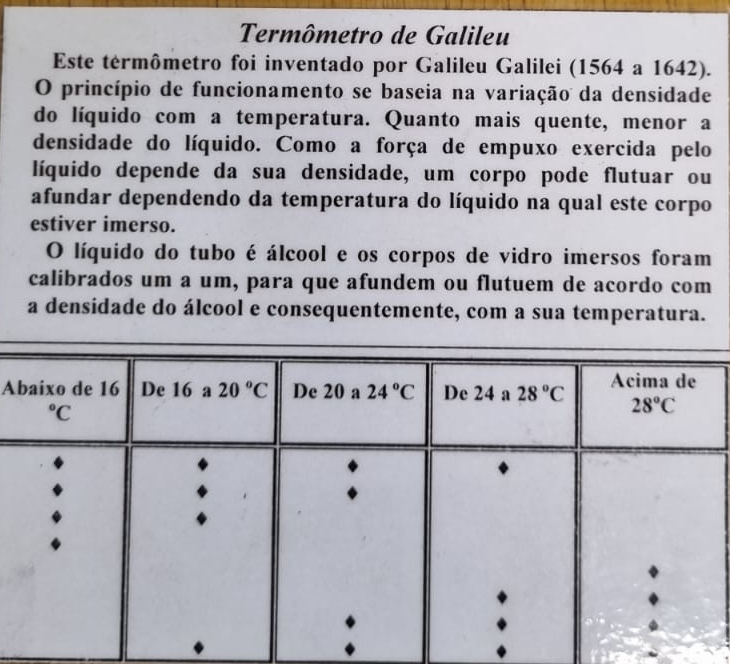
\includegraphics[width=.5\linewidth]{fig/temps}
    \caption{Temperaturas nominais e posições esperadas dos bonecos para cada uma}\label{temps}
\end{figure}

De toda forma, o princípio por trás deste experimento é a variação da densidade do líquido com a variação da temperatura. Ao aquecer, as moléculas que compõe o líquido têm maior energia cinética, aumentando, em média, a distância entre as moléculas do líquido. Desta forma, um objeto submerso no líquido está sujeito à força de empuxo deste, por sua vez, a força de empuxo varia com a densidade do líquido. Ao aumentar a temperatura a densidade do líquido diminui. Por consequência, aumento na temperatura resulta em diminuição da força de empuxo. Como os bonecos também estão sujeitos à força gravitacional, atuando sobre eles sem variação, na mesma direção e em sentido oposto ao da força de empuxo, ao diminuir a força de empuxo a força resultante se torna não nula e faz com que o boneco afunde um pouco mais. O contrário acontece ao resfriar o líquido. 

O termômetro de Galileu é um precursor engenhoso dos termômetros de mercúrio. Uma vantagem interessante deste em relação ao anterior é que não depende do uso de metais pesados. Porém, a resolução do termômetro de galileu depende de ajustar densidades muito próximas entre os objetos de medida, os bonecos no nosso caso. Além disso, o alcance de temperaturas mensuráveis com um termômetro de Galileu é limitado a variações de temperatura na escala da temperatura ambiente (\qty{10}{\celsius}--\qty{36}{\celsius}), não pode medir temperaturas próximas à temperatura de ebulição ou fusão do líquido utilizado. 

\subsection{Psicrômetro}
Foi constatado que o termômetro seco media \qty{25}{\celsius} e o termômetro molhado media aproximadamente \qty{22}{\celsius}. Ao consultar a tabela, temos que a diferença de temperatura é \qty{3}{\celsius}, portanto, umidade de \qty{76}{\percent} a \qty{77}{\percent} na sala. Durante este dia, a temperatura indicada pela previsão do tempo registrada no dia era de \qty{25}{\celsius} enquanto a umidade média no Butantã era de \qty{66}{\percent}. A diferença entre a umidade medida e a umidade média da região é provavelmente decorrente da arborização. Enquanto o campus da USP é bem arborizado e próximo ao rio Pinheiros e à raia, é de se esperar que seja uma região com pico de umidade do ar. 

O princípio por trás do psicrômetro é a termodinâmica. Em particular o equilíbrio de fases. Em todos os momentos, a água está sob pressão do vapor de água e sob agitação em decorrência da temperatura, portanto, o ponto de equilíbrio ocorre quando a pressão de vapor é tal que a quantidade de cada fase fique em equilíbrio dinâmico, o sistema tende à este ponto de equilíbrio. Pensando molecularmente, embora a temperatura seja uma medida da energia cinética média das moléculas de água a real distribuição da energia cinética é caótica e em determinados momentos há moléculas com mais energia cinética que as demais. Se a energia cinética de uma molécula é tal que supere a energia potencial que a atrai às outras moléculas de água, fazendo-a compor a fração líquida, então esta molécula pode se desprender e passar a compor a fração gasosa. 

Se a pressão de vapor for menor do que a pressão de equilíbrio para aquela temperatura, será recorrente que as moléculas se desprendam e evaporem sem condensar novamente. Durante o processo de evaporação, a água toma calor do termômetro, fazendo o medir temperatura mais fria do que o termômetro exposto ao ar. Como justificado, a variação da temperatura deve depender da umidade relativa do ar. Similarmente, se a concentração de moléculas de água no ar for tal que a pressão de vapor exercida sobre a gaze seja igual a pressão de vapor de equilíbrio, então não haverá evaporação e a diferença de temperatura será nula, indicando umidade relativa do ar de \qty{100}{\percent}. Ou seja, qualquer acréscimo de moléculas de água na fase gasosa resulta em condensação. Este é o mesmo fenômeno observado quando há formação de orvalho.

O psicrômetro de dois bulbos é prático por não depender de energia elétrica e ser fácil de carregar. Pode medir a umidade relativa de forma tão sensível quanto for a escala dos termômetros e da tabela. Visto que a pressão de vapor de equilíbrio pode ser determinada para cada temperatura. Como desvantagem, idealmente o psicrômetro é construído com água destilada para evitar variações no equilíbrio por composição química da água. Além disso, o alcance das medidas é limitado para temperaturas em que a água se mantenha líquida, dificultando utilizá-lo para medir umidade do ar em dias com temperaturas abaixo de zero. Por fim, é preciso manter a gaze sempre em contato com uma fonte de água destilada.

